\todo{Overall I find the motivation section to be disconnected -- you need to
make the connection from incremental VM to frontend analysis, and then to the
need to compile these long-running queries to motivate the confluence.}
\todo{Also make the point that this section surveys the state-of-the-art both
from a research perspective and from an implementation experience perspective.}

In a database system, views are one of the central features in attaining both
logical data independence and efficient performance as evidenced by their use
from query optimization to data integration. While it is clear that improvements
in view maintenance techniques would have a significant impact on a number of
database internals challenges, our form of multilevel views and its realization
as efficient low-level code allows us to provide high-performance, lightweight
monitoring and notification services to the benefit of a wide range of
application domains. Consider the following uses:

\begin{list}{\labelenumi}{\usecounter{enumi} \leftmargin=1em}
\addtolength{\itemsep}{-0.5\baselineskip}
\item An automated stock market trading system monitors the distribution of buy
and sell orders of a particular stock to identify the best time and price for
its own orders.

\item A corporate data warehouse monitors the current status of its production
facilities, warehoused inventory and active demand for its products in order to
preemptively identify supply chain problems.

\item A compute cluster monitors its current status overnight to alert a network
administrator when some of its hardware fails, but only if a distributed task
running on the cluster is at risk of becoming unavailable.
\end{list}

These are all use cases of frontend analysis systems to drive rapid
decision-making and actions in contrast to backend OLAP data warehouses for deep
ad-hoc exploratory querying. These kinds of analysis systems sit on the critical
datapath as close as possible to data sources, inspect events on the fly as part
of alert or automated systems often without human intervention, and are key to
operation or to achieving a competitive advantage. Other examples of application
domains include regulatory compliance~\cite{basel2}, fraud
detection~\cite{ibmfico}, computational
advertising~\cite{agarwal2010forecasting}, steered scientific
simulations~\cite{hey2009fourth} and parameter exploration, disaster
prediction~\cite{scholz1973earthquake}, and online machine
learning~\cite{olesen2008real} amongst others.

Many of the above application domains make heavy use of data management tools,
and while traditional OLTP and OLAP systems are not naturally architected for
dynamic aggregation-heavy analysis queries, it is less clear as to why stream
and complex event, and active database technologies are ill-suited for such
workloads. In addition to discussing the architectural mismatches in stream and
trigger-oriented approaches, we present a preliminary experiment across a range
of query processing engines to demonstrate the update, and view refresh rates
they can attain.

\begin{figure*}[htbp]
\begin{tabular}{|l|l|l|l|l|l|}
\hline
Query & \#joins \& types & Predicate types
      & Group bys & Max subquery depth & Description
\\
\hline
Axfinder        & & & & & \\
Brokerspread    & & & & & \\
Brokervariance  & & & & & \\
Missedtrades    & & & & & \\
Pricespread     & & & & & \\
VWAP            & & & & & \\
Q3              & & & & & \\
Q11             & & & & & \\
Q17             & & & & & \\
Q18             & & & & & \\
Q22             & & & & & \\
SSB4            & & & & & \\
Serverload      & & & & & \\
\hline
\end{tabular}
\caption{Features of the algorithmic trading, online decision support, and
cluster monitoring query workload used throughout the experimental evaluations
in this work}
\label{fig:queries}
\end{figure*}


\subsection{Query Workloads for Monitoring}
The above use cases are examples common scenarios in algorithmic trading on
order books, online decision support at a manufacturer, datacenter and network
infrastructure monitoring. 
These update-intensive monitoring applications intrinsically use aggregations
and summarizations, however considering them as flat
select-project-join-aggregate queries is an oversimplification.
In particular, monitoring queries frequently compute a variety of statistics and
compare and contrast them prior to taking action. This leads to queries with
complex dataflows consisting of disjunctions, joins with inequality predicates,
and nested and correlated subqueries composed in arbitrary fashion amongst other
features. We use a query workload drawn from these domains throughout this
paper. \note{We list the salient features of our query workload in terms of
their query processing properties in Figure~\ref{fig:queries}, while their SQL
descriptions are listed in Appendix~\ref{app:queries}.}

The algorithmic trading queries operate on two order book tables consisting of
the buy and sell order books present at an electronic stock exchange -- in the
case of our dataset, over a day's worth of orders for the MSFT symbol on NASDAQ
(approx. 2.5 million orders). The online decision support queries are taken from
the TPC-H benchmark, and processed over a update stream replayed in randomized
order from a TPC-H scale factor \todo{0.1} dataset. One additional query in this
scenario is the \todo{SSB4} query that is inspired by the query 4.2 from the
Star Schema Benchmark modified to work on a TPC-H dataset by using one extra
join operation. The cluster monitoring query operates on a synthetic dataset
that simulates tasks running on a 1000 node cluster.

\todo{More description of query workload, i.e. just verbalize table contents?}

We evaluated this workload on four data management systems, including two stream
processing engines and two popular DBMS, with an open-source (Esper, Postgres)
and commercial implementation (CSPE, CDB)\footnote{We anonymize both of the
commercial systems due to licensing restrictions on publishing benchmarks.} for
each case. We describe implementation specifics below when discussing the
architectural properties of triggers and stream engines. We provide further
details, for example our system specification, with our in-depth experiments in
Section~\ref{sec:experiments}. Figure~\ref{fig:enginecomp} shows the view
maintenance performance achieved by these query processors.
\todo{Check for overlap with experiments section}

\subsection{Incremental View Maintenance}
\begin{itemize}
  \item Postgres has no incremental view maintenance algorithms.
  \item Could not use any incremental view maintenance in our CDB. In fact we
  looked over all the major commercial DBMS and found that none could support
  incremental refresh for the majority of our workload due to their use of
  correlated subqueries, and other features. Most commercial implementations of
  view maintenance algorithms have a long list of restrictions.
\end{itemize}

\subsection{Triggers and Active Databases}

Active database methods and their realization as trigger mechanisms in DBMS
allow us to manipulate database state such as indexes and views in a reactive
manner as DML statements execute. Triggers can be implemented in a variety of
procedural languages from plpgsql, scripting languages such as Python or Perl,
to Java or C. In the case of procedural SQL languages, triggers undergo the same
compilation path as user-defined queries, that is they are compiled into
physical query plans that are interpreted by the query executor.

Triggers exemplifies update processing where the developer looses the ability
for declarative development, and where along with user-defined functions and
aggregates, compilers and query optimizers reside in silos inside a DBMS. Indeed
much of the literature from the database community has focused on issues such as
cascading, recursion and feedback in trigger systems, with limited
(single-level) work on incremental processing that has primarily been drawn from
incremental view maintenance research.

Using triggers, we implemented a full refresh approach to maintain views for our
query workload. We call this approach \textit{repetitive} processing, where on
each update, a post-update trigger re-evaluates the query from scratch. This
approach incurs minimal developer overhead in performing view maintenance. In
our experience, implementing multilevel view maintenance by hand becomes
impractical very quickly (after even one level of delta transformation) due to
the complexity and number of subqueries that arise, affirming the benefits of
automatic incrementalization in a compiler. \todo{Lines of code reference here.}

\begin{itemize}
  \item Set-at-a-time internals vs tuple-at-a-time.
  \item Experiment takeaways 
\end{itemize}


\subsection{Stream and Complex Event Processing}

\begin{itemize}
  \item Inapplicability of windows.
  \item Lack of standard semantics across stream engines, also observed by
  others. Each stream system requires its own implementation and they are not
  portable.
  \item For the CSPE our general strategy: maintain full history with in-memory
  tables, fully replay from in-memory store approaches as updates arrive.
  Essentially turns tables into streams, and then wires together query plan with
  pure-streaming operators. This is essentially like writing iterator based code
  for the entire query (with declarative queries, in the fashion as writing
  trigger code in plpgsql, T-SQL or PLSQL) once the stream is fully replayed.
  \item Experiences:
  \item Esper supports nested queries, but yields inconsistent views over them.
  \item Lack of transactional semantics when updating tables, locking. Counting
  and barrier based approaches
  \item Avoid locking with single-threaded sequential execution and relying on
  deterministic fully pipelined execution of both Esper and CSPE.
  \item Experiment takeaways:
\end{itemize}


\begin{figure}[htbp]
\begin{center}
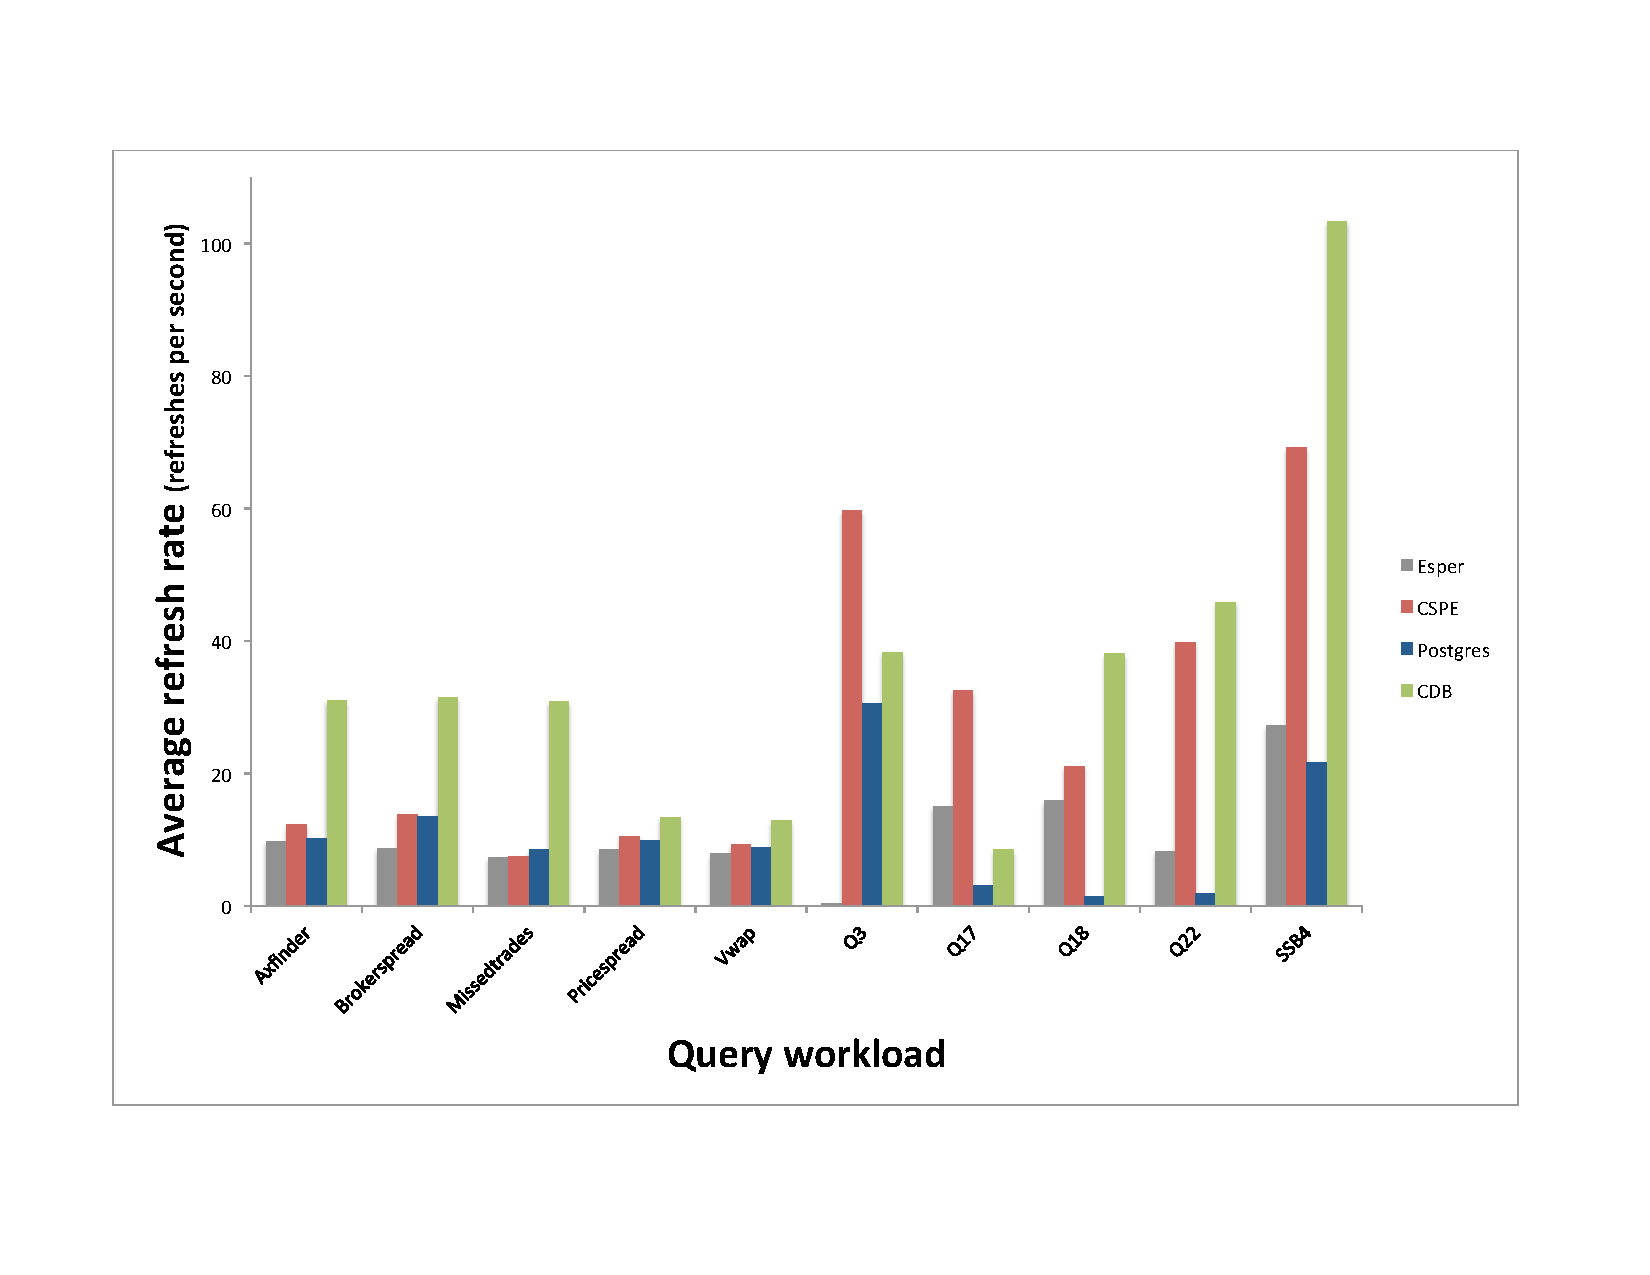
\includegraphics[scale=0.33]{../graphs/graphs/engine-comparison.pdf}
\end{center}
\vspace{-4mm}
\caption{A comparison of four query processing engines to implement view
maintenance, including both open-source and commercial stream engines and DBMS.
All engines perform a full view refresh on update arrival.}
\label{fig:enginecomp}
\end{figure}
